\chapter{Efficient Multi-version Execution}
\label{chap:efficient-execution}

% Recent years have seen a growing interest in using diversity as a way
% to increase the reliability and security of software systems.  One
% form of software diversity that has attracted significant interest
% from the research community is the idea of running multiple
% diversified versions of a program in parallel in order to survive bugs
% and detect security attacks.  In essence, diversity can offer
% probabilistic guarantees that at least one variant survives a bug, or
% that a security attack will be flagged by divergent behaviour across
% variants.

% On the reliability side, which forms the main focus of this paper,
% these diversified versions are either automatically-generated
% variants, multiple versions of the same application, or different
% programs implementing the same interface.  For example, one may run in
% parallel multiple variants that employ complementary thread schedules
% to survive concurrency errors~\cite{compl-schedules11}, multiple
% versions of the same software to survive update bugs~\cite{mx}, or
% multiple web browsers to benefit from the fact that many errors do not
% affect all browser implementations~\cite{cocktail}.  In this paper, we
% show that running multiple versions in parallel can be used in other
% reliability scenarios, such as running expensive error detectors
% (``sanitizers'') during deployment.

% On the security side, these diversified variants are constructed in
% such a way as to reduce the probability of an attack succeeding in all
% of
% them~\cite{cox2006,orchestra09,diehard06,tightlip,capizzi08,devries10,cocktail,trachsel10}.
% For example, one may generate versions with a different arrangement of
% memory blocks in the address space~\cite{diehard06}, or with stacks
% growing in opposite directions~\cite{orchestra09}, to prevent attacks
% whose success depends on the memory layout.

% To enable these scenarios, a monitor process coordinates the parallel
% execution of these variants\footnote{The terms \textit{version} and
%   \textit{variant} are used interchangeably.} and synchronises their
% execution, making them appear as a single application to any outside
% entities.  While synchronisation can be performed at different levels,
% the most common approach is to do it at the level of system calls, for
% two main reasons: first, many existing diversification
% transformations, such as the ones discussed above, 
% % address-space layout randomisation~\cite{diehard06} and
% % instruction-set randomisation~\cite{instr-set-rand03}
% do not change the sequence of system calls (the program's
% \textit{external behaviour}), and the ordering is often preserved even
% across different software versions~\cite{mx}.  Second, system calls
% are the main way in which the application communicates with the
% outside environment, and therefore
% %% the ultimate target of attackers.  Finally, as the main
% %% communication mechanism between applications and the environment,
% %% system calls
% must be virtualised in order to enable the multiple versions to act as
% one to the outside world.

The main challenge in implementing a system call monitor the trade-off between
performance, security, flexibility and ease of debugging.  Many
implementations~\cite{orchestra09,mx,process-replicae07} use the
\lstinline`ptrace` mechanism offered by most UNIX-based operating systems.
While \lstinline`ptrace` has its advantages as show in
Chapter~\ref{chap:safe-updates}, namely ease-of-use and not requiring kernel
modifications, \lstinline`ptrace` introduces large overhead, and these systems
see performance degradations of up to two orders of magnitude.  A much faster
approach is to implement the monitor in kernel space~\cite{cox2006}, but this
requires kernel patches and/or new kernel modules, and the monitor must be run
in privileged mode.  Furthermore, none of these approaches scales well with the
number of variants (as the monitor is both a communication and synchronisation
bottleneck), none are debug-friendly (\lstinline`ptrace` disallows the use of
\gdb, while kernel debugging has its well-known set of limitations) and none of
them have been designed to be flexible with respect to small variations in
system call sequences (which can occur for certain diversification
transformations and across program versions).

In this chapter, we propose \varan,\footnote{\varan's name comes from
  the scientific name \emph{Varanus}, commonly known as the
  \emph{monitor} lizard. Varan is also a name of the Kaiju monster
  that first appeared in the 1958 movie \emph{Varan the
    Unbelievable}.} a novel architecture for implementing multi-version
monitors.  \varan monitors operate at the system call level, run in
user space (and therefore in unprivileged mode), introduce a small
performance overhead for popular C10k network servers and often a
negligible overhead for CPU-bound applications, scale well with the
number of versions, and provide a flexible mechanism for handling small
divergences in the system call sequences issued across versions.

\section{Overview}
\label{sec:overview}

Two key aspects influence the performance and flexibility of an NVX
system: system call interception and version coordination.  We discuss
each in turn below.

\subsection{System call interception}
\label{sec:interception}

%% \begin{enumerate}[(i)]
%% \item wait for the interrupt signaling the entry to a system call;
%% \item examine the registers to determine whether the system
%% call is of interest;
%% \item for any arguments passed by reference, copy the content of
%% the memory for the process address space if necessary;
%% \item if the system call is to be skipped (or performed by the monitor
%% on behalf of the application), replace the original system call with a
%% "null" system call (\ie \lstinline`getpid`);
%% \item restart the execution of the application to execute the system call;
%% \item wait for the interrupt signaling the exit from a system call;
%% \item obtain the process registers to read the system call return value;
%% \item for any output arguments, copy the referenced data from
%% the process address space if needed; and
%% \item continue the execution of the application.
%% \end{enumerate}

The biggest downside of existing system call monitors based on the
\ptrace interface is the high performance
overhead~\cite{orchestra09,tachyon12}.  For each system call
performed by each version, execution must switch to the monitor
process, which has to perform several additional system calls in order
%to be notified about system call entry and exit, 
to copy buffers to and from the version being monitored, nullify the
system call, \etc

For CPU-intensive applications which perform few system calls, this
overhead will be amortised, translating into a modest overall
slowdown.  However, for heavily I/O-bound applications, the slowdown
can be up to two orders of magnitude, which is unacceptable for many
real-world deployments.
%
Consequently, in order to implement a system call monitor with
acceptable overhead even for heavily I/O-bound applications, we need
to eliminate context switching to the monitor and back during
interception and eliminate the need for additional system calls.  
This is accomplished through a combination of selective binary
rewriting and an interprocess communication mechanism based on a
fast shared memory ring buffer.

%\vspace{0.1in} \noindent \textbf{Selective binary rewriting.}  
Whenever code is loaded into memory, \varan scans each code page to
selectively rewrite all system calls with jump instructions to dedicated
handlers.  Section \ref{sec:rewriting} discusses in detail the main
steps and challenges associated with this binary rewriting approach.

To eliminate the need for additional system calls during interception,
\varan uses a shared ring buffer to communicate between versions.  This
ring buffer is heavily optimised for performance: it is stored in
memory, allows largely lock-free communication, and does not require
the dispatch of events to different queues.  These aspects are
discussed in detail in Section~\ref{sec:streaming}.



\subsection{Event-streaming architecture}
\label{sec:coordination}

In prior NVX systems, versions are typically run in lockstep, with a
centralised monitor coordinating and virtualising their execution.
Essentially, at each system call, the versions pass control to the
monitor, which waits until all versions reach the same system call.
Once this happens, the monitor executes the system call and
communicates the result to each individual version.  If two or more
versions try to break the lockstep by executing different system
calls, the monitor needs to either terminate the entire application or
continue executing a subset of the versions in lockstep.

This approach has two key disadvantages.  First, the centralised
monitor is a bottleneck, which can have a significant impact on
performance.  Note that in addition to the synchronisation overhead,
this centralised monitor makes the NVX application execute at the
speed of the slowest individual version.

Second, this approach is totally inflexible to any divergence in the
sequence of system calls executed across versions.  This is an issue
both when running automatically-diversified variants, where certain
transformations may affect the external behaviour, and when running
existing software revisions, where changes in the sequences of
system calls can occur between revisions. 

\begin{figure}[t]
  \begin{center}
    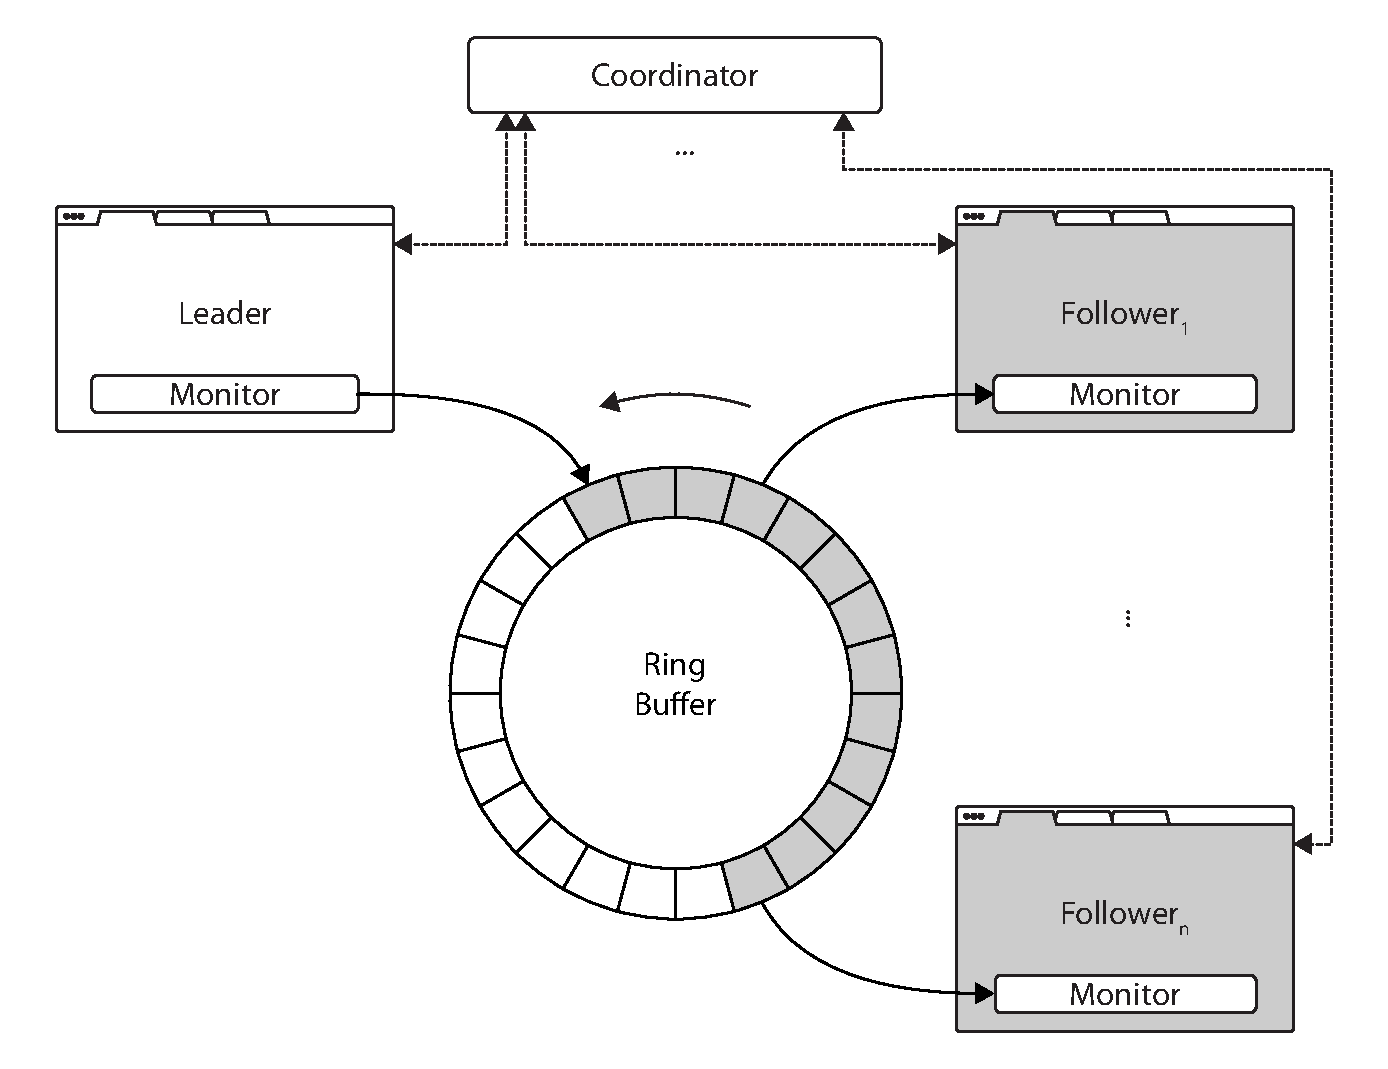
\includegraphics[width=0.6\textwidth]{efficient-execution/figures/architecture}
    \caption{The event-streaming architecture of \varan.}
    \label{fig:architecture}
  \end{center}
\end{figure}

To address these limitations, \varan uses a new approach which we call
\emph{event streaming}.  In this decentralised architecture,
depicted in Figure~\ref{fig:architecture}, one of the
versions is designated as the \textit{leader}, while the others are
\textit{followers}. During execution, the leader records all events into a
shared ring buffer, which are later read by followers to mimic the leader's
external behaviour (\S\ref{sec:streaming}). Events consist primarily
of regular system
call invocations, but also of signals, process forks (\ie \lstinline`clone`
and \lstinline`fork` system calls) and exits (\ie \lstinline`exit` and
\lstinline`exit_group` system calls).

In general, any version can be the leader, although in some situations
some may be a better choice than others--\eg when running multiple
software revisions in parallel, one might prefer to designate the
newest one as leader.  However, the leader can be easily replaced if
necessary, \eg if it crashes (\S\ref{sec:leader-repl}).

The only centralised component in this architecture is the
\textit{coordinator}, whose main job is to prepare the versions for
execution and establish the necessary communication channels.  At a
high level, the coordinator first loads the variants into memory,
injects several special handlers and memory objects into their address
spaces, rewrites any system calls in their code with jumps to the
special handlers and then starts executing the variants
(\S\ref{sec:setup}) in a decentralised manner.

%% recorded by one application version are shortly replayed
%% (\textit{streamed}) to the others, which keeps the log small, as
%% events which have been replayed by all versions can be discarded.
%% Similarly, the NVX context allows for the log to be kept in memory,
%% and for the replay to be done incrementally, with significant
%% performance advantages.  Event streaming is discussed in detail in
%% Section~\ref{sec:streaming}.


%% This is a variant of record-replay~\cite{scribe,jockey,geels06,r2},
%% but the NVX context allows us to overcome two of the main limitations
%% of traditional record-replay techniques, namely (1)~the
%% rapidly-growing log size, especially for system call-intensive
%% applications; and (2)~the long time necessary to replay the execution.
%% Because the multiple versions are executed concurrently, events
%% recorded by one application version are shortly replayed
%% (\textit{streamed}) to the others, which keeps the log small, as
%% events which have been replayed by all versions can be discarded.
%% Similarly, the NVX context allows for the log to be kept in memory,
%% and for the replay to be done incrementally, with significant
%% performance advantages.  Event streaming is discussed in detail in
%% Section~\ref{sec:streaming}.


\subsection{Rewrite rules for system call sequences}
\label{sec:rw}

In addition to eliminating the central monitor bottleneck, our
event-streaming architecture also supports (small) divergences between
the system call sequences of different variants.  For example,
different software revisions can be run inside a classical NVX
system only as long as they all issue the same sequence of system
calls~\cite{mx}.  However, software patches sometimes change the
external behavior of an application.  In particular, many divergences
in system call traces fall into the following two categories:
\begin{inparaenum}[(i)]
\item \emph{addition/removal}, characterising situations when one of
  the versions performs (or conversely does not perform) an additional
  system call, typically as a consequence of an additional check, and
\item \emph{coalescing}, covering the situations when a (repeated)
  sequence of system calls is executed a different number of times in
  each version (\eg one version might execute two \lstinline`write`
  system calls, while another version executes only one
  \lstinline`write` system call to write the same bytes because extra
  buffering is used).

\end{inparaenum}

% \begin{description}
%   \item[Addition/Removal] This class characterises situations when one
%     of the versions performs an additional system call (or conversely
%     does not perform), typically as a consequence of an additional
%     check.
%   \item[Coalescing] This class covers the situations when a (repeated)
%     sequence of system calls is executed a different number of times
%     in each version.  E.g., one version might execute two \lstinline`write`
%     system calls, while another a single equivalent \lstinline`write` to
%     write the same bytes (\eg because extra buffering is used).  
% \end{description}

\varan is the first NVX system that is able to deal with such changes.
When followers process the event sequence streamed by the leader, they
can rewrite it to account for any such differences: \eg they can skip
and merge system calls, or perform some calls themselves.  We provide
a flexible implementation of such rewrite rules using Berkeley Packet
Filters (\S\ref{sec:patternmatching}).


\section{Prototype}
\label{sec:prototype}

%% \begin{figure}[t]
%%   \begin{center}
%%     \includegraphics[width=\columnwidth]{figures/process-model}
%%     \caption{\varan process model.}
%%     \label{fig:process_model}
%%   \end{center}
%% \end{figure}

\begin{figure}[t]
  \begin{center}
    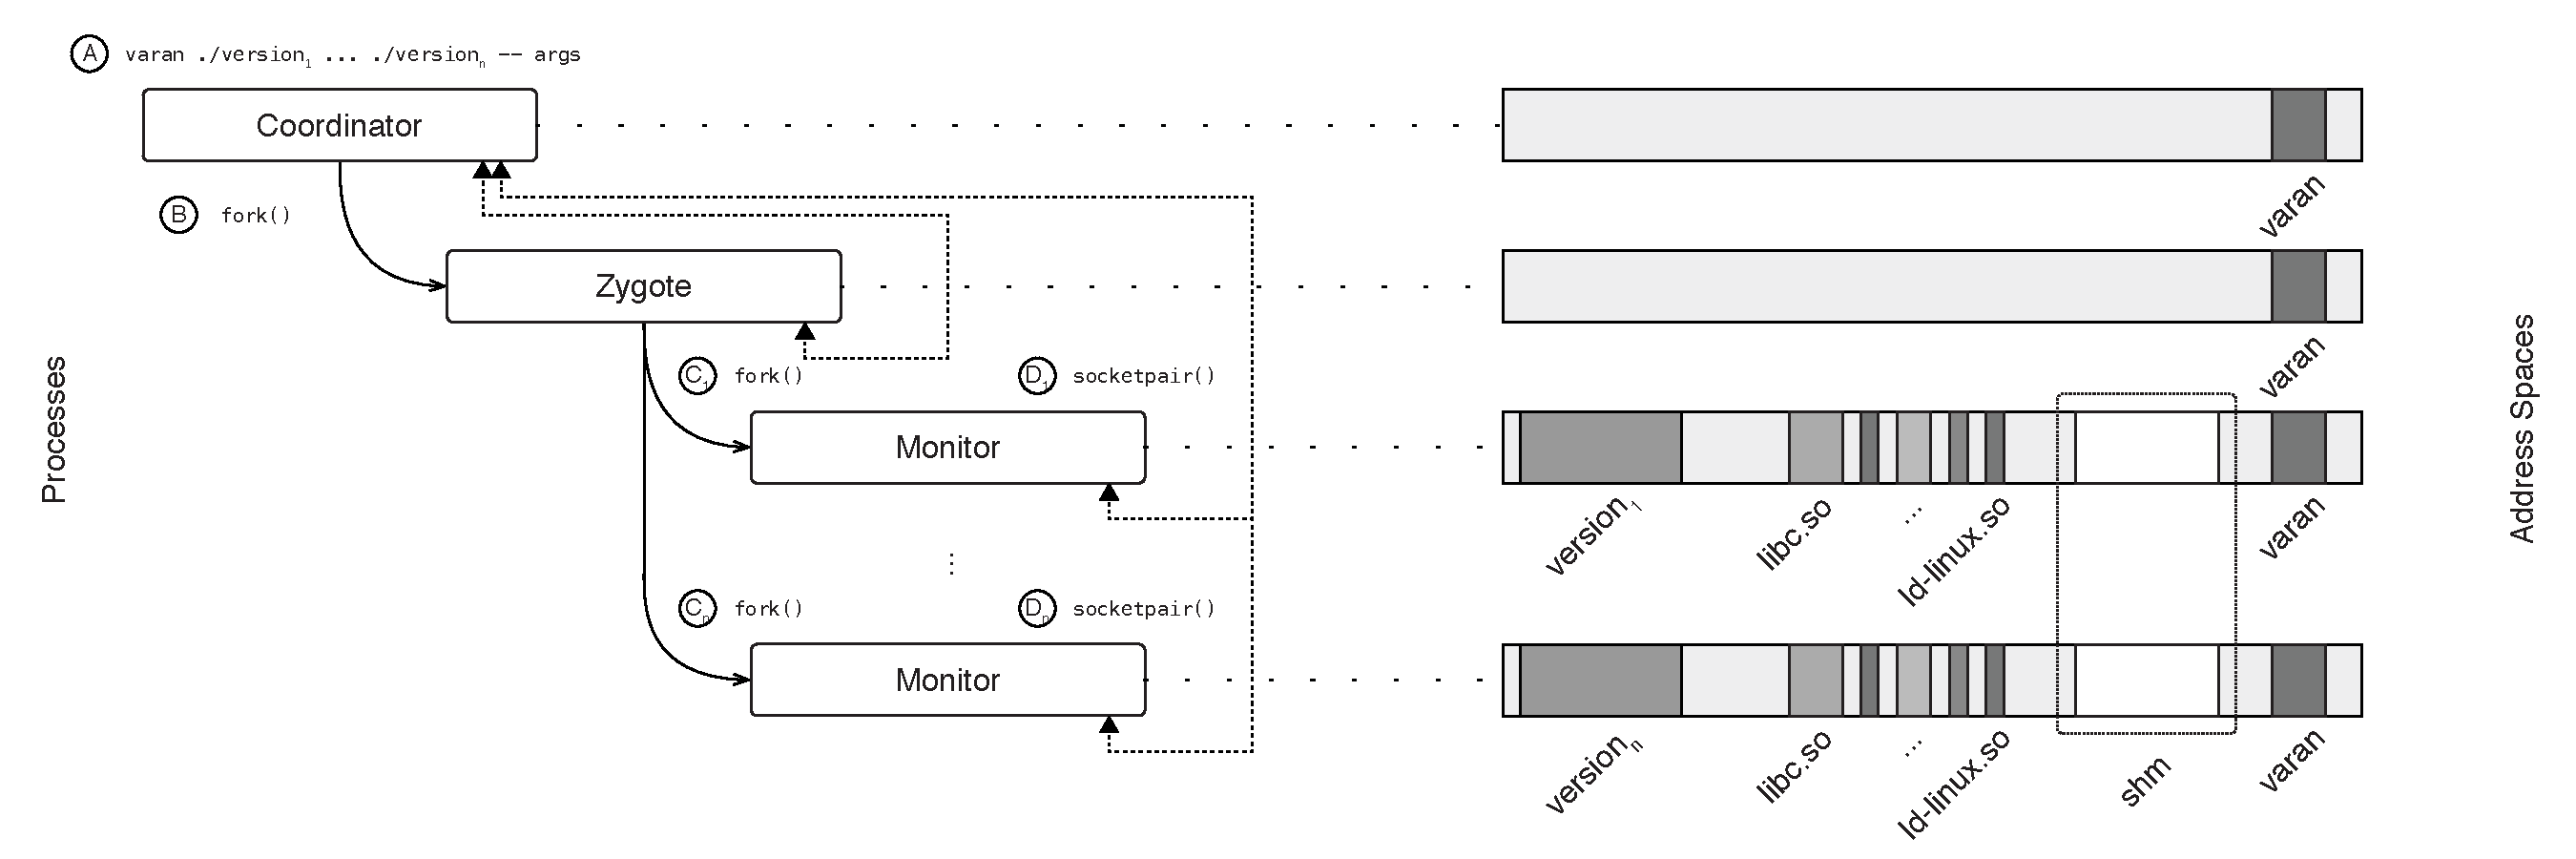
\includegraphics[width=0.75\textwidth]{efficient-execution/figures/address-space}
    \caption{Setup of address spaces and communication channels.}
    \label{fig:setup}
  \end{center}
\end{figure}


We have implemented our approach in a prototype (to which we will also
refer as \varan), targeted at multi-core processors running x86-64 Linux.
\varan works on off-the-shelf binaries (both stripped and unstripped)
and supports single- as well as multi-threaded applications.

When it starts, \varan first sets up the address spaces of all program
versions and establishes the needed communication channels
(\S\ref{sec:setup}).  It then performs selective binary rewriting to
replace all system calls with  jump instructions
(\S\ref{sec:rewriting}).  After these initial stages, the event
streamer component of \varan ensures the coordination of the leader and
its followers (\S\ref{sec:streaming}).


\subsection{Setup of address spaces and communication channels}
\label{sec:setup}

The main steps involved in the setup of version address spaces and the
needed communication channels are shown in Figure~\ref{fig:setup}.  To
run multiple versions in parallel, the user launches \varan's
\emph{coordinator} providing the paths to all versions, together with
any command line arguments required to start them (Step \circl{A} in
Figure~\ref{fig:setup}).

% \begin{lstlisting}[language=bash,numbers=none]
% varan -p /path/to/executable1 
%         -p /path/to/executable2 -- args
% \end{lstlisting}

%The coordinator is linked with the \varan library (\varanlib, stored in
%\lstinline`libvaran.so`), which will be also injected inside each version.
%\varanlib is built as a statically-linked, position-independent library,
%to make sure it does not stand in the way of any segments which have
%to be loaded by the application at fixed addresses.

The \emph{coordinator} first creates the shared memory segment
used for communication among versions, and then spawns the
\textit{zygote} process (\circl{B}), which is responsible for starting
the individual versions. The coordinator communicates with the zygote
via a UNIX domain socket. For each version $i$ that needs to be spawned,
the coordinator sends a fork request to the zygote over this socket
pair, which includes the path to that version executable, the command
line arguments, and the end-point of a socket pair which will be used
for the subsequent communication between the coordinator and that
version (\circl{C$_i$}).
%
After receiving this request, the zygote spawns a new process, which
first finalises the communication with the coordinator
(\circl{D$_i$}).  The coordinator then sends the shared memory
segment descriptor to this process, which maps it inside its address
space.

%% returns a process identifier to the coordinator.  The coordinator then
%% sends the rank and shared memory segment descriptor to the version.

In the final step, the new process starts executing inside the monitor
code, which loads the specified ELF executable and sets up the initial
address space as described in the ELF headers. If the program requires
a dynamic linker, \varan loads the linker image specified in the
header as well.
%% Afterwards, \varan attaches the shared memory segment and initialises
%% the system call table based on the rank and arguments provided by
%% the coordinator.
The text segments of both the application and the dynamic linker are
then processed by the binary rewriter (\S\ref{sec:rewriting}). Finally,
\varan jumps to the application entry point as specified in the ELF header,
starting the execution of the application version.

The right-hand side of Figure~\ref{fig:setup} shows the address spaces
of the coordinator, zygote, and program versions.  When run with
\varan, program versions have two new segments mapped into their
address spaces: the shared memory segment used for communication among
versions (``shm'') and the \varan statically-linked library
(``varan'').  Note that \varan does not prevent address-space layout
randomisation schemes to be used by the operating system.

%% \varan is operates at the thin boundary between the operating system and
%% the user-space application---\ie below the C library and the dynamic
%% linker---and lives inside the address space of the host application;
%% however, the application itself is unaware of its existence.

% The rest of this section provides some extra details regarding the
% role and implementation of the coordinator, monitor and zygote.

\boldtext{Coordinator.}  To set up the address spaces of the versions,
the coordinator acts as a specialized preloader, inspired by
\emph{rtldi}.\footnote{\url{http://www.bitwagon.com/rtldi/rtldi.html}}
However, the coordinator does not attempt to replace the existing
dynamic linker, which would be unnecessarily complex and may affect
compatibility with existing applications. Instead, it simply
intercepts the system calls performed by the linker to enable the
binary rewriter (\S\ref{sec:rewriting}) to rewrite the code of
dynamically-linked shared libraries.  One important advantage of our
interception mechanism is that we do not make use of \ptrace to
intercept calls to the dynamic linker---instead, the binary rewriter
is used to rewrite all the system calls done by the linker with jumps
into the coordinator code.  As a result, \varan can be used in
combination with existing \lstinline`ptrace`-based tools such as \gdb
or \textit{strace}, which greatly simplifies debugging.

%% This also has an advantage of supporting arbitrary dynamic linkers,
%% not just the one provided by GNU C library, albeit it is going to be
%% the most common target.

%% This architecture has several advantages over other commonly
%% approaches. \varan does not require the use of dynamic linker, as
%% required by \lstinline`LD\_PRELOAD`. 



\boldtext{Zygote.} The role of the zygote is to spawn new processes on
request from the coordinator.  Zygote processes are already used in
systems such as \textit{Android} and
\textit{Chrome}~\cite{linuxzygote}---in this paper, we use the term to
refer to the architectural pattern rather than a particular implementation, as \varan
provides its own clean-slate implementation.  While it would be
technically possible for the coordinator to create the processes in
which versions run, this would bring some complications regarding the
communication channels: for example, the second version spawned would
inherit the communication channel between the first version and the
coordinator, which would be undesirable.

\boldtext{Monitor.} The monitor code is built as a statically-linked,
position-independent library, to make sure it does not stand in the
way of any segments which have to be loaded by the application at
fixed addresses.  To ensure that the code can be compiled like this,
we must avoid using any global variables (\ie those in the
\lstinline`.data` section). One consequence is that \varan
cannot use any of the existing C libraries such as \textit{GNU C
  Library}, as these are not typically built to support this
requirement.  Instead, \varan provides its own implementation of the
necessary C library functions based on the \textit{Bionic C
  library}.\footnote{\url{https://android.googlesource.com/platform/bionic}}
To support the use of Linux system calls, \varan uses a modified
version of the \lstinline`linux_syscall_support.h`
header.\footnote{\url{https://code.google.com/p/linux-syscall-support/}}

%% \varanlib provides its own entry point (\ie the \lstinline`\_start` function),
%% which is the starting point for \varan's execution. After start, it first
%% processes the arguments passed on stack by the Linux kernel, including
%% program arguments, environment variables and most importantly the
%% auxiliary data. Then, it loads the specified ELF executable into the
%% address space. Since \varan operates as a pre-loader, it is responsible
%% for setting up the initial address space layout as described by the
%% program header. If the program being executed requires dynamic linker,
%% \varan loads the linker image specified in the program header as
%% well. The text segments of both the application and the dynamic linker
%% are then processed by the binary rewriter (\S\ref{sec:rewriting}).


%% After start, \varan sets up the communication subsystem (\ie the shared
%% memory allocator, the ring buffer) and then forks the Zygote
%% process. The Zygote closes all open descriptors except for the socket
%% used as a communication channel with the coordinator and enters the
%% dispatch loop to wait for incoming requests. On fork request, the
%% Zygote receives command line arguments (\ie \lstinline`argv`) and a set of
%% file descriptors which will be available to the new process; then
%% forks itself and resumes to dispatch loop. The other type of requests
%% that Zygote supports are querying for process status (\ie equivalent
%% of \lstinline`waitpid`) and process termination (\ie \lstinline`SIGKILL`).

%% \begin{structure}
%% \item Establishing the initial memory layout as specified by the ELF
%% binary
%% \item Loading the dynamic loader (if specified by the ELF header)
%% \item Jumping to the application (or dynamic loader) entry point
%% \end{structure}


\subsection{Binary Rewriting}
\label{sec:rewriting}

%% \begin{structure}
%% \item Scanning each text segment in the program address space
%% \item Rewriting every syscall with jump instruction where possible,
%% otherwise using interrupt
%% \item Using table of system call handlers to interpose on selected
%% system calls
%% \end{structure}

To intercept system calls, \varan uses selective binary
rewriting~\cite{bird}. Unlike traditional dynamic binary rewriting
implemented by tools like DynamoRIO~\cite{dynamorio02} or
Pin~\cite{pin05}, where the entire process image is being rewritten,
often introducing a significant performance overhead, \varan only
replaces the instructions for performing system calls (\ie
\lstinline[language={[x64]Assembler}]`int $0x80` on x86 and
\lstinline[language={[x64]Assembler}]`syscall` on x86-64).
%% This approach has been originally implemented in
%% \emph{BIRD}~\cite{bird} for the Windows/x86 platform and later in
%% \emph{seccompsandbox}\footnote{\url{https://code.google.com/p/seccompsandbox/}}
%% for Linux. 
%Our implementation extends the \emph{seccompsandbox}\footnote{\url{https://code.google.com/p/seccompsandbox/}} framework for Linux.

The rewriting itself is done when a segment is mapped into memory with
executable permissions, or an existing memory segment is marked as
executable.  
%(\ie \lstinline`mmap` system calls with executable flag, typically
%performed by the dynamic linker).
During rewriting, \varan scans the segment searching for system call
instructions using a simple x86 disassembler.  Every system call found
is rewritten with a jump to an internal system call entry point. This
process is complicated by the fact that while a system call
instruction is only one byte long, a jump instruction requires five
bytes.  Therefore, in order to rewrite the system call with a jump, we
also need to relocate some of the instructions surrounding the system
call---\ie perform binary detouring via trampolines~\cite{detours}.
On the rare occasions when this is not possible (\eg because the
surrounding instructions are potential branch targets), we replace the
system call with an interrupt (\lstinline`INT 0x0`).  This interrupt
is handled by \varan through a signal handler installed during
initialisation, which redirects the control flow to the system call
entry point as for other system calls.

The system call entry point first saves all registers, and then
consults an internal system call table to check whether there is a
handler installed for that particular system call; if so, it calls
that handler, otherwise it invokes the default handler.  After
processing the system call, the entry point handler restores all
registers and returns to the original caller (using
\lstinline`sigreturn` in the case of system calls intercepted via an
interrupt). The system call entry point also implements support for
restarting system calls (\ie signaled by the \lstinline`-ERESTARTSYS`
error code). This is used in certain scenarios supported by \varan
such as transparent failover (\S\ref{sec:failover}).

The internal system call table can be easily changed to accommodate
various application scenarios.  In particular, the only difference
between the leader and the followers is the system call table. For
example, the \lstinline`write` system call would be redirected in the leader
to a function that performs the call and records its result in the
shared ring buffer, while in the followers it would be redirected to a
function that reads the results from the shared buffer without making
the call.
%% \varan allows both the system call table and the default system call
%% handler to be provided by the embedder of \varan \todo{Where shall we
%%   described the possibility of \varan embedding, \ie building tools on
%%   top of \varan?}. This makes it easy to customize \varan behavior for
%% different use cases (\S\ref{sec:failover}). For our prototype, we have
%% provide three different system call tables (\ie record, replay and
%% passthrough). 
\varan  also provides a Python script which can produce new tables
and their implementations using templates.
%% ; in fact, the passthrough table was implemented using this
%% generator. We have also used the generator throughout the \varan
%% development for testing and debugging purposes.

Finally, note that in order to prevent potential attackers to easily inject
system calls into the program, the binary rewriter follows a
W$\mathbin{\oplus}$X discipline throughout execution, making sure that
segments are not marked as both writable and executable at the same
time.


\subsubsection{Virtual System Calls}
\label{sec:vsyscall}

Certain Linux system calls are accelerated through the \emph{vsyscall}
page and the \emph{vDSO} segment. These are mapped into the address
space of each Linux process, and contain system call
implementations. These \textit{virtual system calls} do not incur the
context switch overhead between kernel and user space associated with
standard system calls.

The \emph{vsyscall} page was introduced first, but is being deprecated
in favor of the \emph{vDSO} segment.
%% limitations\footnote{We are referring to x86-64 version, on x86
%%   systems the vDSO segment contains a function used to determine the
%%   preferred method of making a system call}. 
The main reason for this development is that the \emph{vsyscall} page
is mapped to a fixed address, making it susceptible to return-oriented
programming attacks~\cite{ROP:tissec12}. To address this issue, the
vDSO segment is mapped to a random address. Since the segment is
dynamically allocated, it can also support an arbitrary number of
virtual system calls (currently \lstinline`clock_gettime`, \lstinline`getcpu`,
\lstinline`gettimeofday` and \lstinline`time`).

Virtual system calls represents one of the major limitations of
\lstinline`ptrace`-based monitors. Since these system calls are entirely
implemented in user space, they cannot be intercepted via \ptrace.
This is an important limitation: as these system calls provide access
to timing information, they are often used as a source of
non-determinism (\eg for random number generators) and their handling
is critical for any NVX system. %Despite this, previous systems either
%omit discussion on virtual system call handling~\cite{mx,orchestra11}
%or explicitly mention their inability to handle them~\cite{tachyon12}.

To our knowledge, \varan is the first NVX system which handles virtual
system calls, using binary rewriting. 
%In \varan, binary rewriting is also used to intercept virtual system
%calls.
Handling calls made via the \textit{vsyscall} page is easier because
the function symbols are always mapped to the same address.  
%% We can therefore easily identify calls to these functions while
%% scanning the text segment and rewrite them to calls into our system
%% call table.
To handle \textit{vDSO} calls, we first need to determine the base
address of the \textit{vDSO} segment; this address is passed by the
kernel in the ELF auxiliary vector via the \lstinline`AT_SYSINFO_EHDR`
flag.\footnote{\url{https://www.gnu.org/software/libc/manual/html_node/Auxiliary-Vector.html}}
Second, we need to examine the ELF headers of the \textit{vDSO}
segment to find all symbols.  Identifying calls to these symbols is
more complicated than in the \textit{vsyscall} case because these
symbols are allocated at arbitrary addresses.  Instead, we replace the
entry point of each function with a jump to dynamically generated code
which sets up the stack and then issues a call to the \varan system
call entry point as in the case of regular system calls. Furthermore, we
provide a trampoline, which allows the invocation of the original
function, by moving the first few instructions of each function to a
new place, followed by a jump to the original code. This allows \varan
to take advantage of the virtual system call mechanism to further
improve performance.

%% Finally, we note that this function interception mechanism is not
%% specific to system calls and can be used to intercept arbitrary
%% functions in the target application if needed, similarly to
%% Detours~\cite{detours}.



\subsection{Event Streaming}
\label{sec:streaming}

%% \begin{structure}
%% \item Externally observable behavior triggers events (\eg system calls,
%% signals), these events are being recorded and replayed by individual
%% versions
%% \item The concept of event-streaming; all versions share a common event
%% stream (\ie log) of fixed size
%% \item One version is always elected as a leader adding new events to the
%% stream, the other versions are followers replaying the events from the
%% stream
%% \item When the leader crashes, followers elect a new leader
%% \end{structure}

As we discussed briefly in Section~\ref{sec:overview} and illustrated
graphically in Figure~\ref{fig:architecture}, the leader records all
external events into a shared ring buffer, while the followers replay
them to mimic the leader's behavior. The leader is the only version
interacting with the environment, \ie executing the system calls, with
the exception of system calls which are local to the process (\eg
\lstinline`mmap`). % or \lstinline`sigaction`).

As in any NVX system operating at the level of system calls, \varan
has to be aware of the system call semantics, in order to transfer the
arguments and results of each system call.  \varan currently
implements \syscallsHandlers system calls, which were all the system
calls encountered across our benchmarks.\footnote{We configured \varan
  to emit an error message when an unhandled system call is
  encountered, and have implemented system call handlers on demand.}

%% All application instances running in parallel under \varan are assigned
%% ranks, similarly to OpenMPI~\cite{OpenMPI}. The instance\footnote{We
%%   refer to the instances rather than a process as application may have
%%   multiple threads/subprocesses} with rank 0 is denoted as
%% \emph{leader} while all other instances are denoted as
%% \emph{followers}. 


%% When followers would execute a system call under normal execution, now
%% they simply return a value from the event stream (\ie the return value
%% of the system call executed by the leader).

% \varan recognizes several different types of events:
% \begin{inparaenum}[(i)]
% \item \emph{syscall} for the system call entry,
% \item \emph{sysret} for the system call exit,
% \item \emph{signal} for an interceptable signal,
% \item \emph{exit} for the process exit.
% \end{inparaenum}
% Furthermore, it is possible to add other types of events if necessary.

%% Each event has a fixed size of 64 bytes where first byte is
%% used as an event type.  The size has been deliberately chosen to be
%% fit into a single cache line on modern x86 CPU (see \S\ref{sec:ipc}
%% for more details).

%% \subsection{Interprocess Communication}
%% \label{sec:ipc}

%% \begin{structure}
%% \item Sending events from one process to other without the use of system
%% calls to avoid the additional overhead
%% \item Shared memory queues for process to process communication
%% \item Custom shared memory allocator with reference counting
%% \end{structure}

%% Since one of our primary goals for \varan was to minimize the performance
%% overhead, to avoid additional system calls being made during system
%% call handling (\S\ref{sec:overview}), we have designed an interprocess
%% communication mechanism which does not use system calls (\eg
%% socket-based communication primitives).

\subsubsection{Shared ring buffer}
\label{sec:ring}

For fast communication, the leader and its followers share a common
ring buffer of fixed size, which is held entirely in memory.  Our
initial solution used a separate shared queue for each
process~\cite{fastforward,mcringbuffer}, with the
%% Shared memory queues are often used for fast core-to-core
%% communication in high-performance applications.
coordinator acting as an event pump---reading events from the leader's
queue and dispatching them into followers' queues.  This approach
worked well for a low system call rate, but at higher rates the event
pump quickly became a bottleneck.  
% Furthermore, although we used a
% state-of-the-art shared queue implementation~\cite{bqueue}, we still
% experienced a large performance overhead for system call
% interception---over $20\times$ for a worst-case microbenchmark,
% compared to $4\times$ in the final implementation.

As a result, we have instead opted for a design based on the Disruptor
pattern~\cite{disruptor}, which uses a shared ring buffer allowing concurrent
access by multiple producers and consumers, eliminating the need to dispatch
events among queues, and thus improving both performance and memory
consumption.  Our implementation uses C11 atomics, 
%introduced in C11 and now supported by both GCC and Clang, 
in combination with cache aligning to
achieve maximum performance with minimal use of locking (locks are used only
during memory allocation and deallocation).

%The ring buffer is used to stream events between processes.  
The size of the ring \varan uses is configurable and has a default
value of 256 events.  Each event has a fixed size of 64 bytes; the
size has been deliberately chosen to fit into a single cache line on
modern x86 CPUs.  This is sufficient for sending signals and system
calls for which all arguments are passed by value (on x86-64, a system
call can have up to six arguments of eight bytes, to fit into general
purpose registers).  However, for system call arguments passed by
reference, the payload might have variable size and can be potentially
larger than the event itself.  In this case, we use events only to
transfer shared pointers, which identify memory shared across
versions.

The use of a shared memory buffer may result in a waste of system
resources when the leader process performs a system call which blocks
for a long period of time, as the followers use busy waiting to check
for new events. To address this problem, we have introduced the
concept of a \emph{waitlock}. Whenever a follower makes a blocking
system call, it acquires the waitlock. If there is no event available,
the thread will block until the leader wakes up and notifies it. The
waitlocks are efficiently implemented using a combination of C11
atomics and futexes~\cite{futex}.

\subsubsection{Transferring file descriptors and leader replacement}
\label{sec:leader-repl}

Apart from the ring buffer, each version has a \textit{data channel},
implemented using UNIX domain sockets.
% Together, the ring buffer and data channel form an \emph{event
% stream} which is a primary communication mechanism for exchanging
% events among instances.
The data channel is used to send information which cannot be
transferred via shared memory, in particular open file descriptors.
Whenever the leader obtains a new file descriptor (\eg by opening a
file), it sends this descriptor to all followers, effectively
duplicating the descriptor into their processes. This is a crucial
mechanism which enables the leader to be replaced transparently when
it crashes. When the leader crashes, the follower that is elected as
the new leader can simply continue executing using existing
descriptors (\eg responding to requests coming over the network)
without any disruption of service.

% Currently, UNIX domain sockets do not support broadcast, so the leader
% communicates with the followers via the coordinator, which then sends
% the descriptor separately to all followers.  However, there are
% proposals to add broadcast support for UNIX domain
% sockets,\footnote{\url{https://lkml.org/lkml/2012/2/20/208}} which would
% simplify the design of our prototype and further improve performance.


\subsubsection{Multi-process and multi-threaded applications}
\label{sec:threading}
\label{sec:ipc}

Handling processes and threads is crucial in supporting many modern
applications.  
%The discussion below refers to processes, but threads are handled in a
%similar way.
In our design, we have opted to have separate ring buffers for each
tuple of processes or threads in the system: for instance, when a
process forks, the parent processes in the leader and all followers
form one tuple, and the child processes another, with a process in
each tuple acting as the leader.  More exactly, when a new process is
forked, a new socket pair is established between the process and the
coordinator and a new ring buffer is allocated.  The leader then
continues execution, but the coordinator waits until all followers
fork a new process, establishing appropriate socket pairs for
communication, and setting the child processes to read events from the
newly-allocated ring buffer.

To alleviate non-determinism issues due to scheduling, \varan enforces
system call ordering across all tuples using Lamport's
\emph{happens-before} relation~\cite{lamport78}. Currently, this is
only implemented for multi-threaded applications, which make intensive
use of synchronisation primitives, but the same solution could be
employed for multi-process applications too.

\begin{figure}[t]
  \begin{center}
    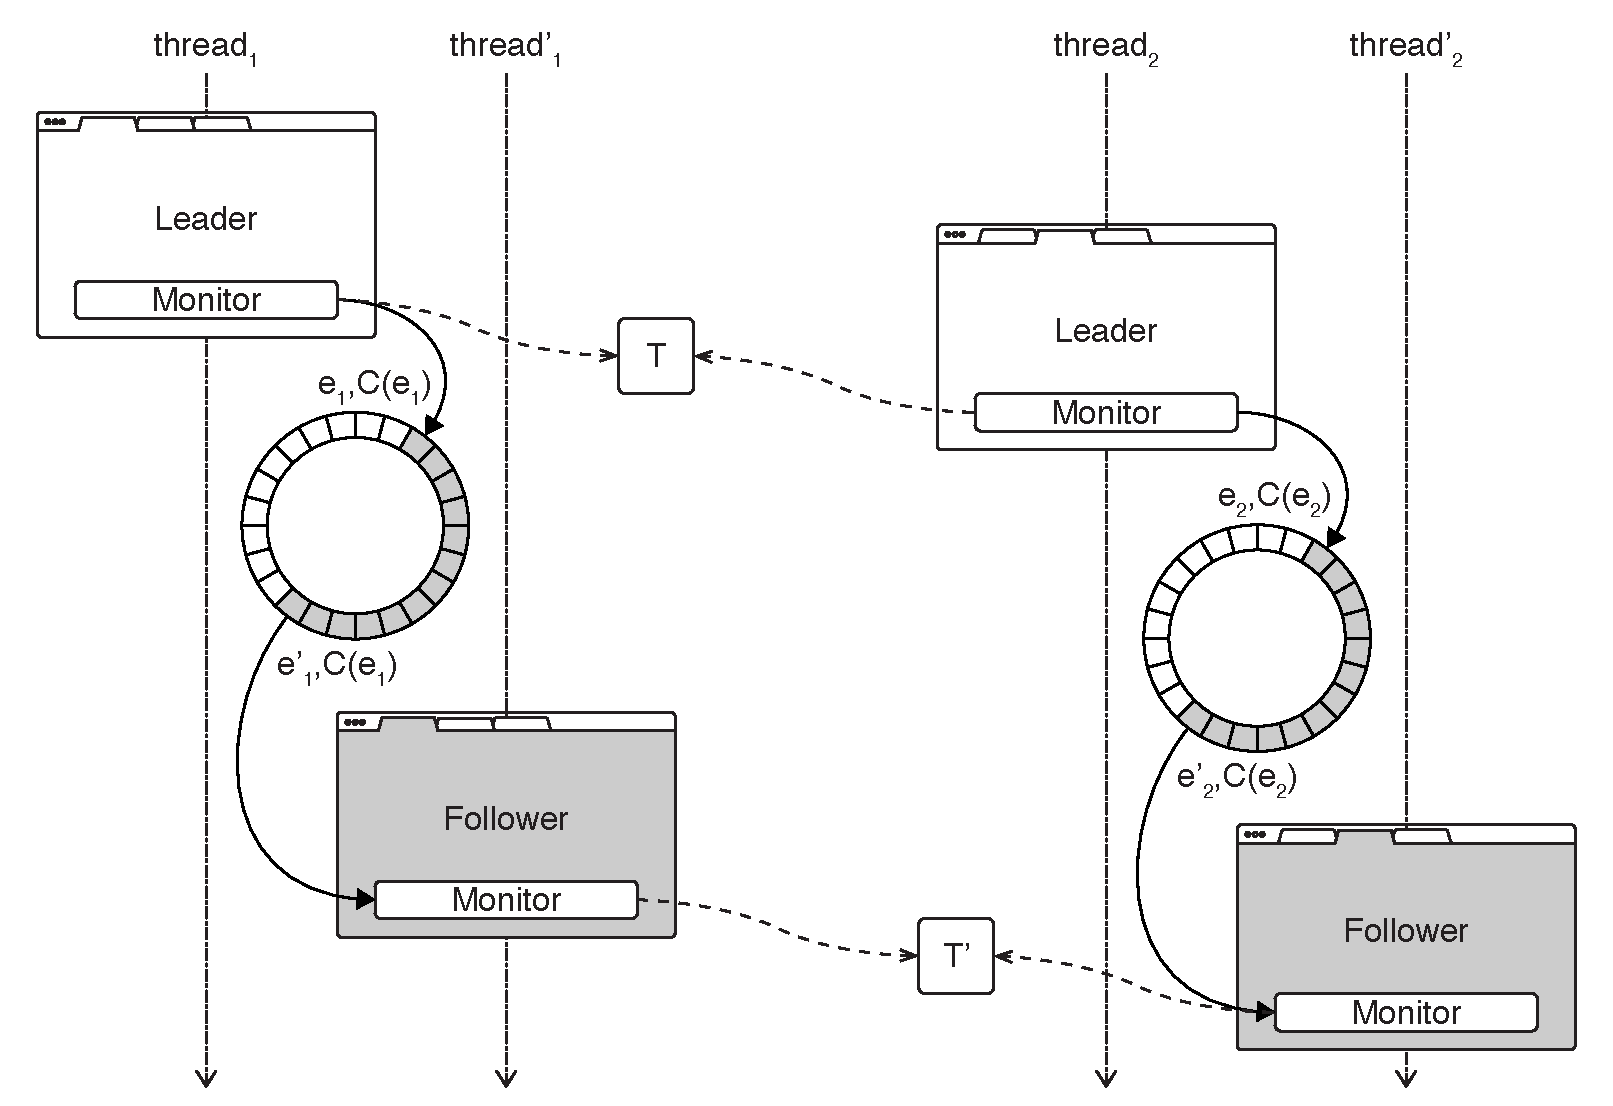
\includegraphics[width=0.75\textwidth]{efficient-execution/figures/multithreading}
    \caption{Event delivery in a multi-threaded NVX program, with
      the ordering of events enforced using logical clocks.}
    \label{fig:multithreaded}
  \end{center}
\end{figure}

Each variant has an internal Lamport clock, shared by all threads, and
each event $e_i$ sent through the ring buffer is annotated with a
timestamp $C(e_i)$.  Then, when replaying events from the buffer, each
thread checks the timestamp of every new event and only receives the
event if it does not violate the happens-before relation. This
scenario is depicted in Figure~\ref{fig:multithreaded}. If $e_1\to
e_2$ ($e_1$ happens before $e_2$), then $C(e_1)<C(e_2)$ and \varan
enforces $e'_1\to e'_2$. Without the ordering, there could be a
situation where $e_1\to e_2$, but $e'_1\not\to e'_2$, which could lead
to a divergence. A similar approach has been proposed in the past for
record-replay in shared-memory systems~\cite{levrouw94}.

To implement the internal clocks shared by the threads of a variant
($T$ and $T'$ in Figure~\ref{fig:multithreaded}),
we use an atomic counter allocated in the shared memory space and
updated using C11 atomics for efficiency.  When the leader thread
writes a new event into the ring buffer, it increments its variant's
clock value and attaches it to the event.  When a follower thread
reads an event from the ring buffer, it compares its variant's clock
value with the event's timestamp.  If they are equal, the thread
increments its variant's clock value and processes the event,
otherwise it continues waiting. Our current implementation uses busy
waiting, as the wait times are expected to be small.  However, shall
this become a problem in the future, it is possible to use blocking
wait instead (\eg a futex).

% Since Disruptor (\S\ref{sec:ring})
% allows concurrent writes by multiple producers without the need for
% expensive synchronisation, the use of a single shared buffer does not
% create a performance bottleneck. %hinder the application performance.

Our solution resembles existing deterministic multi-threading (DMT)
mechanisms~\cite{coredet:asplos10,dthreads:sosp11}. The guarantees
provided by \varan are weaker than those typically provided by these
systems as we do not enforce ordering across atomics-based
synchronisation primitives. We have not detected any system call
divergences caused by related data races in our benchmarks, which
include multi-threaded applications (\eg \redis), similar to the
experience reported for prior NVX systems. However, shall this become
a problem, we could address it by employing a stronger form of
determinism similar to existing DMT systems.

%
% However, this weaker form of determinism
% does not typically pose a problem for real-world applications as long
% as they are properly synchronised.  Note that data races resulting
% from missing or incorrect synchronisation can cause followers to issue
% a different sequence of system calls from the leader.  If this
% happens, we could either try to apply one of the rewriting rules
% (\S\ref{sec:patternmatching}), or terminate the follower.
%

%% Each instance also has a dedicated \emph{service channel}, similarly
%% to the data channel implemented using UNIX domain sockets. The service
%% channel is used to transfer commands and service requests between
%% coordinator and the instance.

%% One such example are \lstinline`fork` and \lstinline`clone` system calls. The new
%% process spawned as a result of these system calls needs to have its
%% own data and service channel. The parent process is responsible for
%% creating these using a \lstinline`sockepair` system call. One end of each
%% pair is inherited by the new process while the other end is sent to
%% the coordinator where it is associated with the new process.

%Note that data races resulting from missing or incorrect
%synchronisation can cause followers to issue a different sequence of
%system calls from the leader.  If this happens, that follower would
%have to be terminated.  We first note that \varan has not detected any
%system call divergences caused by data races in our benchmarks (which
%include many popular applications such as \apache, \nginx, and \redis),
%so this might not be such an important aspect in practice.  Prior NVX
%systems do not address this problem either, likely due to a comparable
%experience.

%However, we envision two possible solutions.  The first one would be
%to use deterministic multi-threading (\eg
%Dthreads~\cite{dthreads:sosp11}).  The second solution would be to
%allow developers to document any benign races as rewrite rules
%(cf. \S\ref{sec:patternmatching}).

\subsubsection{Memory allocation scheme}  

Efficient shared memory allocation plays an important role in a system
like \varan.  We use a custom shared memory pool allocator implementation.
%, similar to the one used by OpenMPI.\footnote{\url{http://www.open-mpi.org/}}
The allocator has the notion of buckets for different allocation sizes,
where each bucket holds a list of segments, and each segment is
divided into chunks of the same size; each bucket holds a free list of
chunks.  When there are no more unused chunks in a bucket, the
allocator requests a new segment from the memory pool, and divides it
into chunks which are then added to the free list. Each bucket also
has a lock associated with it which has to be held prior to an
allocation from that bucket. 
% While this design is relatively simple,
% it performed well in our benchmarks. We also experimented with
% more advanced designs (\eg using different allocation strategies for
% smaller and larger blocks), but the basic allocator always
% outperformed all other implementations.  

%% However, we believe it might still be possible to come with a more
%% specialized allocation strategy which would further improve the
%% performance of \varan, and this is something we would like to address in
%% our future work.

%% The critical part of many systems which use shared memory for
%% communication is deallocation. There are various solutions to this
%% problem. One possibility is to use some form of garbage collection,
%% such as reference counting. Unfortunately, this solution is not
%% applicable in our case since the leader is not aware of any of the
%% consumers processing its events making it difficult to consistently
%% manage the reference counts. The original Disruptor implementation,
%% which targets the Java runtime simply relied on the garbage collector
%% provided by the virtual machine. Unfortunately, this solution is not
%% applicable in our case either. Instead, we have extended the C-based
%% Disruptor implementation to notify a follower if it is the last one
%% that processes an event. \todo{how?}  If that is the case, the
%% follower is responsible for freeing the associated memory. This
%% solution does not add any overhead and does not require any
%% modifications to the allocator.

% This property allows us sharing memory between individual application
% instances without explicitly tracking which instance is responsible for
% deallocation, or using the back channel to notify instance that the block is
% available for deallocation as in the case of OpenMPI

\subsection{Rewrite rules for system call sequences}
%\subsubsection{System call filtering and rewriting}
\label{sec:patternmatching}

\varan uses Berkeley Packet Filters (BPF)~\cite{bpf} to implement the system call
rewrite rules introduced in Section~\ref{sec:rw}.  BPF is a machine
language for writing rules and an interpreter shipped with many UNIX
implementations, including Linux and BSD.  BPF filters have been
traditionally used to filter network packets, but recently also for
system call filtering as a part of seccomp ``mode 2'' (also known as
seccomp-bpf).

We have integrated a BPF interpreter in \varan to allow for system
call rewrite rules. Our implementation is based on the Linux kernel
code which was ported to user space and extended for NVX
execution. \varan provides BPF extensions on top of the instruction
set used by seccomp-bpf.\footnote{\url{https://www.kernel.org/doc/Documentation/networking/filter.txt}}
The \lstinline[language={[bpf]Assembler}]`event` extension allows
access to the event stream, which can be used to compare the system
calls executed across versions, as we will show in
Section~\ref{sec:mv-execution}.

%We have also made the offset, used to access the \lstinline`struct seccomp_data` content writable.

% This required adding a new return value
% \lstinline`SECCOMP_RET_REPLACE` where the bottom 16-bits of the return
% value specify the new system call number the original system call is
% going to be rewritten to.  Since these extensions does not add any new
% instructions or extend the semantics of the BPF language, the
% \lstinline`bpf_asm` tool can be used to compile the filters into a
% binary form. This can be then loaded into \varan on start through a
% command line option.


The use of BPF has a number of advantages.  First, it does not require
the user to modify and recompile the monitor on every rule
change. This is particularly important as rewrite rules can be
application specific. Second, the BPF machine language was designed to
be simple enough to prevent certain classes of errors---in particular,
all filters are statically verified when loaded to ensure termination.
% (\ie every filter has to end with a \lstinline`ret` instruction).



%We also argue that the choice of BPF as a language for stream rewriting rules
%makes it easier to adopt by administrators, the most likely users of \varan,
%compared to some other more esoteric languages such as Haskell~\cite{tachyon}.

%% \begin{lstlisting}{language=[bpf]Assembler,caption={Example of a BPF rewriting rule}}
%% ld [0]                /* offsetof(struct seccomp_data, nr) */
%% jne #1, good          /* __NR_write */
%% bad: ret #0           /* SECCOMP_RET_KILL */
%% ldi #18               /* __NR_pwrite */
%% add #0x00070000       /* 18 + 0x00070000 */
%% ret %a                /* SECCOMP_RET_REWRITE */
%% good: ret #0x7fff0000 /* SECCOMP_RET_ALLOW */
%% \end{lstlisting}

\section{Performance evaluation}
\label{sec:evaluation}

One of the main contributions of \varan is a significantly lower
performance overhead compared to existing state-of-the-art NVX
systems.  Therefore, we have conducted an extensive performance
evaluation, using microbenchmarks (\S\ref{sec:microbenchmarks}),
high-performance C10k servers (\S\ref{sec:c10k}) and applications used to
evaluate prior NVX systems (\S\ref{sec:comparison}).

The benchmarks were run on a four-core/eight-thread machine with
a 3.50~GHz Intel Xeon~E3-1280 CPU and 16~GB RAM running 64-bit Ubuntu 14.04
LTS. Both the server and client application on the same machine using the
loopback device to ensure that CPU is fully saturated.
%while the servers were run on a pair of such machines, one
%running the server under \varan and the other the client.  The machines are
%located in the same rack, connected by a 1~Gb Ethernet link.

\subsection{Microbenchmarks}
\label{sec:microbenchmarks}

To measure the overhead introduced by \varan while processing individual
system calls, we designed a series of experiments that compare a
system call intercepted and executed by \varan against the same system
call executed natively. We used five different system calls:

\begin{enumerate}

%\item \lstinline`close` is representative of an inexpensive system call.
%  We invoke it with argument \lstinline`-1`, which returns immediately
%  with an error representing a NOP system call.

\item \lstinline`close(-1)` is representative of an inexpensive system call,
  which returns immediately.

%\item \lstinline`write` is representative of system calls which involve
%  expensive I/O, but whose result can be sent entirely as a single
%  event in the ring buffer.  We invoke the system call to write a
%  512-byte buffer to \lstinline`/dev/null`.

\item \lstinline`write(DEV_NULL, "...", 512)` is representative of system
  calls which involve expensive I/O, but whose result can be sent
  entirely as a single event in the ring buffer.

%\item \lstinline`read` is representative of system calls which involve
%  expensive I/O, and whose result cannot be fully included in the
%  associated event in the ring buffer.  Instead, it has to be copied
%  via additional shared memory (\S\ref{sec:ring}). We invoke the
%  system call to read a 512-byte buffer from \lstinline`/dev/zero`.

\item \lstinline`read(DEV_NULL, "...", 512)` is representative of system calls which
  involve expensive I/O, and whose result cannot be fully included in the
  associated event in the ring buffer.  Instead, it has to be copied via
  additional shared memory (\S\ref{sec:ring}).

%\item \lstinline`open` is representative of system calls that require
%  transferring file descriptors (\S\ref{sec:leader-repl}).  We invoke
%  it with \lstinline`/dev/null` and \lstinline`O\_RDONLY` as arguments.

\item \lstinline`open("/dev/null", O_RDONLY)` is representative of system calls that
  require transferring file descriptors (\S\ref{sec:leader-repl}).

\item \lstinline`time(NULL)` is a virtual system call implemented via the
  \textit{vDSO} segment (\S\ref{sec:vsyscall}). It internally calls
  \lstinline`__vdso_time` (since glibc 2.15).  We could not measure
  the overhead of using the \textit{vsyscall} page, because it is
  deprecated on our system (and all recent versions of Linux), with
  all \textit{vsyscalls} now redirected to their \textit{syscall}
  versions.

\end{enumerate}

%% The \lstinline`open` demonstrates the cost of the file descriptor transfer; we have
%% used the \lstinline`/dev/null` file with \lstinline`O\_RDONLY` flag. \lstinline`read` and
%% \lstinline`write` use the I/O performance overhead, by reading and writing 512B
%% buffer from \lstinline`/dev/zero` and to \lstinline`/dev/null` respectively. The \lstinline`read`
%% is clearly more expensive system call, as it needs to transfer the content of
%% the buffer read using the shared memory (\S\ref{sec:streaming}). The
%% \lstinline`close` system call is a representative of all other cases.

We execute each system call one million times and compute the average
of all execution times.  Time measurements were done using the time
stamp counter (\ie the \lstinline`RDTSC` instruction). Each set of
measurements was preceded by a warm-up stage in which we executed the
system call \num{10000} times. % to warm up the caches.

\begin{figure}[!t]
  \centering
  \includegraphics[width=\textwidth]{efficient-execution/graphs/micro}
  \caption{System call microbenchmarks.}
  \label{fig:micro_syscall}
\end{figure}

%\begin{figure}[!t]
%  \centering
%  \includegraphics[width=\columnwidth]{results/micro_syscall}
%  \caption{System call microbenchmarks.}
%  \label{fig:micro_syscall}
%\end{figure}

Figure~\ref{fig:micro_syscall} shows the results.  The first set of
bars labeled \textit{native} shows the execution time without \varan.
The second set of bars labeled \textit{intercept} shows the execution
time with interception, measuring the cost of binary rewriting: for
these experiments, the intercepted system call is immediately
executed, without any additional processing.  As it can be seen, the
interception cost is small, at under \maxInterceptOvh in all
cases. The overhead of intercepting the virtual system calls is high
in relative terms, but low in absolute ones: \vdsoIntercept vs
\vdsoNative for native execution in case of \lstinline`time`.

The set of bars labeled \textit{leader} shows the execution time for
each system call to be intercepted, executed and recorded by the
leader.  That is, it is the sum of the \textit{intercept} cost and the
cost of recording the system call.  For \lstinline`close` and \lstinline`write`,
the overhead is only \closeLeaderOvh and \writeLeaderOvh respectively
on top of the native execution, because the arguments and results of
these system calls can be recorded in a single event.  For \lstinline`read`,
this is more expensive, at \SI{139}{\percent}, because transferring the result also
involves accessing additional shared memory.  Finally, the cost for
\lstinline`open` is the highest, since it also involves the slower transfer
of the returned file descriptor via a UNIX domain socket.

Finally, the set of bars labelled \textit{follower} shows the execution
time of the follower, which has to intercept each system call and read
its results from the ring buffer and (if necessary) shared memory.  As
expected, the costs for \lstinline`close` and \lstinline`write` are low (and
significantly lower than executing the system call), because the
entire result fits into a single event on the ring buffer. The costs
for \lstinline`read` and \lstinline`open` are higher, because they involve
additional shared memory and transferring a file descriptor,
respectively, but they are still lower than the costs incurred by the
leader.


%\boldtext{vDSO calls.}  We similarly measured the overhead of
%performing a virtual system call via the \textit{vDSO} segment
%(\S\ref{sec:vsyscall}).  The system call used was \lstinline`time`,
%which internally calls \lstinline`\_\_vdso\_time` (since \stt{glibc
%  2.15}).  We could not measure the overhead of using the
%\textit{vsyscall} page, because it is deprecated on our system (and
%all recent versions of Linux), with all \textit{vsyscalls} now
%redirected to their \textit{syscall} versions.

%\begin{figure}[!t]
%  \centering
%  \includegraphics[width=\columnwidth]{results/micro_vsyscall}
%  \caption{vsyscall and vDSO microbenchmarks.}
%  \label{fig:micro_vsyscall}
%\end{figure}

%Figure~\ref{fig:micro_syscall} shows the results, using the same set
%of bars as in Figure~\ref{fig:micro_syscall}.  We have opted this time
%to show absolute numbers, and to include the data for \lstinline`close(-1)`
%from Figure~\ref{fig:micro_syscall} for comparison.  The overhead of
%intercepting the system call is high in relative terms, but low in
%absolute ones: \vdsoIntercept vs \vdsoNative for native execution.
%The \textit{leader} and \textit{follower} costs are similarly high in
%relative terms but low in absolute ones: \vdsoLeader and
%\vdsoFollower, respectively.

\subsection{C10k servers}
\label{sec:c10k}

Existing NVX systems, including those based on \stt{ptrace}, can already
run CPU-bound applications efficiently with overhead typically $<20\%$.
As a result, we focus our evaluation on high-performance, heavily
I/O-bound C10k servers which%
\begin{inparaenum}[(1)]
\item represent the worst-case scenario for a system-call monitor; and
\item form the backbone of modern, highly-scalable web applications, for
  which security and availability are critical.
\end{inparaenum}

The \nservers server applications used in our evaluations are
summarized in Table~\ref{tbl:apps} (the size is measured in lines of
code, as reported by the \stt{cloc} tool). For our performance experiments, we
ran the same version of each application multiple times with different number
of instances (in practice you would typically run different versions). Each
experiment was performed six times, with the first measurement used to warm up
the caches and discarded.  The overhead was calculated as a median of the
remaining five measurements.

\begin{table}
  \centering
\begin{tabular}{lcrl}
  \toprule
  \textsc{Application} & \textsc{Size} & \textsc{Threading} \\
  \midrule
  Beanstalkd & 6,365 & single-threaded \\
  Lighttpd & 38,590 & single-threaded\\
  % Memcached & 9,779 &  multi-threaded\\
  % MongoDB & 898,293 & multi-threaded \\
  Nginx & 101,852 & multi-process\\
  Redis & 34,625 & multi-threaded\\
  \bottomrule
\end{tabular}
  \caption{Server applications used in the evaluation.}
  \label{tbl:apps}
\end{table}

% \begin{figure}[!t]
%   \centering
%   \includegraphics[width=\columnwidth]{results/macro.pdf}
%   \caption{Performance overhead for the \beanstalkd, \lighttpd and \nginx servers for different number of followers.}
%   \label{fig:servers}
% \end{figure}

% \begin{figure*}[!t]
%  \centering
%  \includegraphics[width=0.6\textwidth]{results/c10k.pdf}
%  \caption{Performance overhead for the \beanstalkd, \lighttpd and \nginx servers for different number of followers.}
%  \label{fig:servers}
% \end{figure*}

% \begin{figure*}[!t]
%  \centering
%  \includegraphics[width=0.6\textwidth]{results/macro_redis.pdf}
%  \caption{Performance overhead for \redis operations for different number of followers.}
%  \label{fig:redis}
% \end{figure*}

We give a short overview of each benchmark and the way in which we
measure performance (namely throughput) in our experiments:

\boldtext{\textit{Beanstalkd}} %\footnote{\url{http://kr.github.io/beanstalkd/}}
is a simple and fast work queue, used by a number of websites to
distribute jobs among workers. We used revision \stt{157d88b} from the
official \textit{Git} repository, the latest revision at the time of
writing.  To measure performance, we used
\stt{beanstalkd-benchmark} %\footnote{\url{https://github.com/fangli/beanstalkd-benchmark}}
with $10$ concurrent workers each performing $10,000$ push operations
using $256$ bytes of data per operation.
%The results are summarized in Figure~\ref{fig:macro_beanstalkd}.

\boldtext{\textit{Lighttpd}} %\footnote{\url{http://www.lighttpd.net/}}
is a lightweight web server optimized for high performance
environments. The version used for the measurements was 1.4.36,
the latest version in the 1.4.x series at the time of writing.
We measured the performance of serving a simple HTML webpage using
\stt{wrk}, which was run for $10$s with $10$ clients.

%% \stt{weighttpd}\footnote{\url{https://github.com/lighttpd/weighttp}},
%% which is the benchmarking tool developed by the authors of
%% \lighttpd. We set up \stt{weighttpd} to perform $100,000$ requests,
%% using $10$ concurrent clients running in $2$ threads.
%The results can be seen in Figure~\ref{fig:macro_lighttpd}.


%% \boldtext{\textit{Memcached}}\footnote{\url{http://memcached.org/}} is a
%% high-performance, distributed memory object caching system, used by
%% many high-profile websites to alleviate database load.

%% To measure the performance overhead introduced by \nx when running
%% \memcached, we used \stt{memslap}, a load generation and benchmarking
%% tool for \memcached, which is a part of
%% \stt{libmemcached}.\footnote{\url{http://libmemcached.org/}}

\boldtext{\textit{Nginx}} %\footnote{\url{http://nginx.org/}}
is highly popular reverse proxy server often used as an HTTP web
server, load balancer or cache. We used version 1.5.12, the
latest at the time of writing.  We measured
performance using the same workload as for \lighttpd.

%% measured the performance of serving
%% a simple HTML webpage using
%% \stt{wrk},\footnote{\url{https://github.com/wg/wrk}} which was run for
%% $10$s with $10$ clients.

\boldtext{\textit{Redis}} %\footnote{\url{http://redis.io/}}
is a high-performance in-memory, key-value data store, used by many
well-known services. % such as Twitter, GitHub and StackOverflow.
% Pinterest, Snapchat, Craigslist, Digg, Flickr 
We used version 2.9.11 in our experiments.  To measure
performance, we used
\emph{redis-benchmark}, %\footnote{\url{http://redis.io/topics/benchmarks}}
distributed as a part of Redis. The benchmark issues different types
of commands supported by Redis and measures both the throughput and
the latency for each type. We used the default workload, \ie 50
clients issuing 10,000 requests and calculated and average overhead
across all commands. 

\begin{figure}[!t]
 \centering
 \includegraphics[width=\columnwidth]{efficient-execution/graphs/macro.pdf}
 \caption{Performance overhead for the \beanstalkd, \lighttpd, \nginx and \redis servers for different number of followers.}
 \label{fig:servers}
\end{figure}

The first part of Figure~\ref{fig:servers} shows the results for all servers. All performance
numbers are obtained using the client-side tools presented above.  Since the
client machine is located on the same rack as the server, these numbers
represent a worst-case scenario, as the network latency would hide some of the
overhead for a more distant client machine.

%Figures~\ref{fig:servers} and \ref{fig:redis} show the results for all
%servers.  The results for \redis are shown separately, because \redis
%has 16 different command types.  All performance numbers are obtained
%using the client-side tools presented above.  Since the client machine
%is located on the same rack as the server, these numbers represent a
%worst-case scenario, as the network latency would hide some of the
%overhead for a more distant client machine.

For each benchmark, we show one bar, normalized relative to native
execution, showing the performance of \nx using a given number of
followers.  We stop at six followers, because our machine has eight
threads, and we also need one thread for the leader and one for the
coordinator.  
%For space reasons, for \redis we show results for only 0, 3 and 6 followers.

The set of bars for 0 followers measure the interception overhead
of \nx using binary rewriting.  This overhead is negligible for
\lighttpd and most \redis operations, \nginxIntercept for \nginx, and
\beanstalkdIntercept for \beanstalkd.

For all benchmarks, we see that the performance overhead increases
slightly with the number of followers.  For instance, the overhead for
\beanstalkd increases from \beanstalkdOneFollower for one follower to
\beanstalkdSixFollowers for six followers, while the overhead for
\lighttpd increases from \lighttpdOneFollower to
\lighttpdSixFollowers.

The figure also shows that there is a significant difference across
benchmarks: the worst performer is \beanstalkd, which sees performance
degradations in the range of 55\%-81\%, while the best performers are
\lighttpd, with only 12\%-15\% overhead and some operations in \redis
(not shown separately in Figure~\ref{fig:servers})
%such as \stt{LRANGE\_300}, \stt{LRANGE\_500} and \stt{LRANGE\_600}
with under 3\% overhead.


\subsection{Comparison with prior NVX systems}
\label{sec:comparison}

While Sections~\ref{sec:microbenchmarks} and \ref{sec:c10k} illustrate the
worst-case synthetic and real-world scenarios for a system call monitor, in
order to compare \varan directly with prior NVX systems, we have also run it on
the same set of benchmarks used to evaluate prior systems.  In particular, we
chose to compare against two state-of-the-art NVX systems:
%\strata~\cite{cox2006}, \orchestra~\cite{orchestra09}, and
\tachyon~\cite{tachyon12}.  These systems and their benchmarks are briefly
described  in the first three columns of Table~\ref{tbl:systems}.  To our
knowledge, we are the first to perform an extensive performance comparison of
existing NVX systems.

\begin{table}[t]
\begin{center}
\caption{Existing systems we have compared \varan against.}
\label{tbl:systems}
\begin{tabular}{lllrr}
  \toprule
  \textsc{System} & \textsc{Mechanism} & \textsc{Benchmarks} & \textsc{Overhead} & \textsc{\varan} \\

  \midrule
  \mx~\cite{mx} & ptrace & \lighttpd (http\_load) & \mxLighttpd & \lighttpdHttploadOneFollower \\
                      &  & \redis (redis-benchmark) & \mxRedis & \redisOneFollower \\
                      &  & \speczerosix & \mxSpec & \speczerosixOneFollower \\
  %\hline
  %\strata~\cite{cox2006} & modified kernel & \httpd (WebBench 5.0) & \strataHttpd & \httpdWebBenchOneFollower  \\
  \hline
  \orchestra~\cite{orchestra09} & ptrace & \httpd (ApacheBench)    & \orchestraHttpd & \httpdAbOneFollower  \\
                                &        & \speczerozero & \orchestraSpec & \speczerozeroOneFollower \\
  \hline
  \tachyon~\cite{tachyon12} & ptrace & \lighttpd (ApacheBench) & \tachyonLighttpd & \lighttpdAbOneFollower \\
                            & & \thttpd (ApacheBench) & \tachyonThttpd & \thttpdOneFollower \\
  \bottomrule
\end{tabular}
\end{center}
\end{table}

\begin{figure}[!t]
 \centering
 \includegraphics[width=\textwidth]{efficient-execution/graphs/comparison}
 \caption{Performance overhead for the \httpd, \thttpd, and \lighttpd
   servers for different numbers of followers to allow for comparison
   with existing systems.}
 \label{fig:comparison}
\end{figure}


The last two columns of Table~\ref{tbl:systems} show the cumulative
results.  Since prior systems only handle two versions, the comparison
is done against \varan configured in the same way.  However, we remind
the reader that one of the strengths of \varan's decentralised
architecture is that it can often handle multiple versions with minimum
additional overhead, and below we also show how \varan performs on
these benchmarks when more than two versions are used.

\paragraph{\httpd} \footnote{\url{https://httpd.apache.org/}}
was used by \orchestra.  We used version 1.3.29, the same as in the
original work~\cite{orchestra09}.  The overhead reported for
\orchestra is \orchestraHttpd using the \emph{ApacheBench}
benchmark. \varan introduces \httpdAbOneFollower overhead using the
same benchmark, which is a significant improvement.
Figure~\ref{fig:comparison} shows the overhead introduced by \varan
for \httpd (and the other servers used to evaluate prior work) with
different numbers of followers.  As it can be seen, \varan scales very
well with increasing numbers of followers for these benchmarks.

%was used by both \strata and \orchestra.  We used version 1.3.29
%mentioned by \orchestra (\strata did not report the version used).
%The overhead reported for \orchestra is \orchestraHttpd using the
%\emph{ApacheBench} benchmark and \strataHttpd for \strata using
%\emph{WebBench 5.0}. \varan introduces \httpdWebBenchOneFollower overhead
%using \emph{WebBench} and \httpdAbOneFollower overhead with
%\emph{ApacheBench}, which is an improvement over previous work.

\paragraph{\lighttpd} %\footnote{\url{http://www.lighttpd.net/}}
has been used to evaluate both \mx and \tachyon.  We used version
1.4.36. %(neither \mx nor \tachyon reported the version used). 
\mx used the \emph{http\_load} benchmark and reported \mxLighttpd overhead
while \tachyon used the \emph{ApacheBench} benchmark and reported a
\tachyonLighttpd overhead.  When benchmarked using \emph{http\_load},
\varan introduced only \lighttpdHttploadOneFollower overhead, while with
\emph{ApacheBench} it introduced no noticeable
overhead. %\lighttpdAbOneFollower.  
In both
cases, this marks a significant improvement over previous work.

\paragraph{\thttpd}\footnote{\url{http://www.acme.com/software/thttpd/}}
was shown to introduce \tachyonThttpd overhead when run on top of
\tachyon using the \emph{ApacheBench} benchmark. When run on top of
\varan using the same settings as in \cite{tachyon12}, we have not
measured any noticeable overhead.

\paragraph{\redis} 1.3.8 \footnote{\url{http://redis.io/}}
was used in the evaluation of \mx.  The performance
overhead reported by \mx was \mxRedis using the \lstinline`redis-benchmark`
utility. When run with \varan using the same benchmark and the same workload,
the overhead we measured was \redisOneFollower, which is again a significant
improvement over previous work.

\begin{figure}[!t]
  \centering
  \includegraphics[width=\textwidth]{efficient-execution/graphs/spec2000}
  \caption{\speczerozero performance overhead for different numbers of followers.}
  \label{fig:spec2000}
\end{figure}

\paragraph{\speczerozero}\footnote{\url{http://www.spec.org/cpu2000/}} 
was used to evaluate \orchestra.  We used the latest available version
1.3.1.  \orchestra reported a \orchestraSpec overhead, while \varan
introduced only a \speczerozeroOneFollower overhead. The results for
the individual applications contained in the \speczerozero suite and
for different numbers of followers can be seen in
Figure~\ref{fig:spec2000}. The reason these applications scale poorly
with the number of followers is likely due to memory pressure and
caching effects~\cite{jaleel07}, and to the fact that our machine has
only four physical cores (with two logical cores each).  We plan to
investigate these results in more detail in future work.

\begin{figure}[!t]
  \centering
  \includegraphics[width=\textwidth]{efficient-execution/graphs/spec2006}
  \caption{\speczerosix performance overhead for different numbers of followers.}
  \label{fig:spec2006}
\end{figure}

\paragraph{\speczerosix}\footnote{\url{http://www.spec.org/cpu2006/}}
was previously used to evaluate \mx. We used the latest version 1.2.  The
overhead reported by \mx was \mxSpec, while \varan introduced only
a \speczerosixOneFollower overhead.
Individual results can be seen in Figure~\ref{fig:spec2006}.  


%\begin{figure}[!t]
  %\centering
  %\includegraphics[width=\columnwidth]{results/macro_beanstalkd}
  %\caption{Beanstalkd performance overhead.}
  %\label{fig:macro_beanstalkd}
%\end{figure}

%\begin{figure}[!t]
  %\centering
  %\includegraphics[width=\columnwidth]{results/macro_lighttpd}
  %\caption{Lighttpd performance overhead.}



\section{Transparent failover}
\label{sec:applications}

%NVX systems introduce a variety of opportunities for increasing
%software reliability and availability via transparent failover.  For
%instance, one can run in parallel multiple variants of an application with
%different memory layouts, different software revisions or different
%implementations of a given interface to survive bugs that occur 
%only in some of them.   

The primary application of \varan is \emph{transparent failover}, \ie the
ability to transparently switch over to the non-crashing version in the event
of failure without any disruption in the service.
\varan makes it easy to implement transparent failover.  When one of the
versions crashes, the \lstinline`SIGSEGV` signal handler installed in each
version notifies the coordinator, which decides what restart strategy to use.
When one of the followers crashes, the coordinator unsubscribes it from the
list of currently-running followers, and discards it without affecting other
followers.  When the leader crashes, it designates one of the followers as the
new leader (currently the one with the smallest internal ID), and notifies it
to switch its system call table (\S\ref{sec:rewriting}) to that of the leader,
and to restart the last system call while discarding the old (crashed) leader.

%Furthermore, as an execution
%runtime targeted towards multi-version execution applications, \varan also
%supports running multiple different software versions in parallel.  We discuss
%both of these scenarios in detail below.

To demonstrate support for transparent failover, we reproduced the
\redis bug described in Section~\ref{multi-version:scenarios}.  We ran
in parallel eight consecutive revisions of \redis from the range
\lstinline`9a22de8` to \lstinline`7fb16ba`, where the last revision
introduced a bug which crashes the server by causing a segmentation
fault. We then set up a client to send an \lstinline`HMGET` command that
triggers the bug, and measured the increase in latency for that command.
When the buggy version is a follower, we do not observe any increase in
latency, as expected.  When the buggy version is the leader, the latency
increases from \redisnormallatency to \redisfailoverlatency.  In both
cases, we observed no extra degradation in throughput for the commands
that follow.

This example also demonstrates the difference between \mx and \varan; while \mx
can recover from the crash (\S\ref{sec:redis}) unlike \varan, which
discards the crashing version, \mx can only run two versions in parallel
while \varan can run arbitrary number of versions with lower performance
overhead as shown by the comparison in Section~\ref{sec:comparison}.

As an additional experiment, we ran revisions \lstinline`2437` and
\lstinline`2438` of \lighttpd (also introduced earlier), the latter of
which introduced a crash bug.  We then set up a client that triggers the
bug and measured the latency for that request. Both when the buggy
version was the leader or a follower, there was no significant increase
in latency, which remained at around~\lighttpdnormallatency.
%set up a client that triggers the bug and measured the increase in
%latency for that command. As for the \redis scenario, there is no
%increase in latency when the buggy version is a follower.  When it is
%the leader, the latency increases from \lighttpdnormallatency to
%\lighttpdfailoverlatency.  

\subsection{Handling divergent behaviour}
\label{sec:mv-execution}

\begin{figure}[t]
\begin{center}
\begin{lstlisting}[alsolanguage=diff,numbers=none,label=lst:lighttpd-suid,caption={\lighttpd SUID bit detection patch}]
@@ -66,0 +67,11 @@
+#ifdef HAVE_GETUID
+# ifndef HAVE_ISSETUGID
+
+static int l_issetugid() {
+       return (geteuid() != getuid() || getegid() != getgid());
+}
+
+#  define issetugid l_issetugid
+# endif
+#endif
+
@@ -592 +603 @@ int main (int argc, char **argv) {
-       if (!i_am_root && (geteuid() == 0 || getegid() == 0)) {
+       if (!i_am_root && issetugid()) {
\end{lstlisting}
\end{center}
\end{figure}

Multiple different software versions (revisions) can be run inside an NVX
system as long as they all issue the same sequence of system calls. This
limitation is due to the fact that prior NVX systems run versions in lockstep
(\S\ref{sec:rw}).

Because \varan does not run the versions in lockstep and can use system call
rewrite rules, it can often overcome this limitation. To illustrate, we used
several \lighttpd revisions from our evolution study
(\S\ref{evolution:external}) which introduced new system calls and as such
cannot be run in parallel by prior NVX systems that rely on lockstep execution.

As a first experiment, we ran revision \lstinline`2435` as leader together with
revision \lstinline`2436` as follower. The patch is shown in
Listing~\ref{lst:lighttpd-suid}. Revision \lstinline`2436` introduces two
additional checks using the \lstinline`getuid` and \lstinline`getgid` system
calls.  More precisely, revisions until and including \lstinline`2435` used
\lstinline`geteuid()` and \lstinline`getegid()` C library functions to check
the user account under which the server is being run, before issuing an
\lstinline`open` system call.  This resulted in a sequence of
\lstinline`geteuid`, \lstinline`getegid` and \lstinline`open` system calls.
Revision \lstinline`2436` replaced the use of the aformentioned functions with
\lstinline`issetugid()` which changed the system call sequence to
\lstinline`geteuid`, \lstinline`getuid`, \lstinline`getegid`,
\lstinline`getgid`, followed by \lstinline`open` as before.

To allow for this divergence, we used the custom BPF filter shown in
Listing~\ref{lst:lighttpd}.  The filter is executed by the
follower whenever a divergence is detected.  In our experiment, this
happens when the follower executes the newly introduced
\lstinline`getuid` system call. The filter first loads the system call
number executed by the leader into the implicit BPF accumulator
(line~\ref{line:load-leader}) and checks whether the call is either
\lstinline`getegid` (line~\ref{line:check-getegid}) or
\lstinline`open` (line~\ref{line:check-open}).  The former will be
true in this case, so control will transfer to
line~\ref{line:load-getuid}, which loads the system call number
executed by the follower into the accumulator, checks whether it is
\lstinline`getuid` (line~\ref{line:check-getuid}) and finally
transfers control to line~\ref{line:allow} returning the value
\lstinline`SECCOMP_RET_ALLOW`, which instructs \varan to execute the
additional system call (\ie \lstinline`getuid`) in the follower.  Any
other combination of system calls would have killed the follower
(line~\ref{line:kill}). After executing the \lstinline`getuid` system
call and replaying the execution of \lstinline`getegid` (which the
leader also executed), \varan would detect a second divergence when
the follower tries to execute \lstinline`getgid` instead of
\lstinline`open`. This divergence would be resolved using the same
filter, taking the path on lines~\ref{line:check-open},
\ref{line:load-getgid}, \ref{line:check-getgid} and \ref{line:allow}.

Note this is only one possible filter for allowing this divergence; in
particular, one could write a filter that takes into account more
information about the context in which it should be applied, \eg by
inspecting some system call arguments.

% or more system calls preceding the divergence.

\begin{figure}[t]
\begin{center}
\begin{lstlisting}[label={lst:lighttpd},language={[bpf]Assembler},caption={Example of a BPF rewriting rule.}]
ld event[0] /*@\label{line:load-leader}@*/
jeq #108, getegid       /* __NR_getegid *//*@\label{line:check-getegid}@*/
jeq #2, open            /* __NR_open *//*@\label{line:check-open}@*/
jmp bad
getegid:
ld [0]                  /* offsetof(struct seccomp_data, nr) *//*@\label{line:load-getuid}@*/
jeq #102, good          /* __NR_getuid *//*@\label{line:check-getuid}@*/
open:
ld [0]                  /* offsetof(struct seccomp_data, nr) *//*@\label{line:load-getgid}@*/
jeq #104, good          /* __NR_getgid *//*@\label{line:check-getgid}@*/
bad: ret #0             /* SECCOMP_RET_KILL *//*@\label{line:kill}@*/
good: ret #0x7fff0000   /* SECCOMP_RET_ALLOW *//*@\label{line:allow}@*/
\end{lstlisting}
\end{center}
\end{figure}

%% To translate the filter into bytecode, the user can use the provided
%% \lstinline`vx_bpf` tool and pass the output directly to \varan when starting the
%% application:

%% \begin{lstlisting}[language={bash},numbers=none]
%% vx --filter "$(vx_bpf lighttpd.filter)" \
%%   /path/lighttpd-2435 /path/lighttpd-2436 \
%%   -- -f lighttpd.conf
%% \end{lstlisting}

We used a similar filter to run revisions \lstinline`2523` and
\lstinline`2524`, the latter of which introduces an additional
\lstinline`read` system call to access the \lstinline`/dev/urandom`
file to obtain an additional source of entropy.  We were also able to
run revisions \lstinline`2577` and \lstinline`2578` where the
difference consists of an additional \lstinline`fcntl` system call to
set a \lstinline`FD_CLOEXEC` flag on one of the file descriptors.

Currently, \varan's implementation can use BPF filters only to allow adding
or removing system calls in followers.  However, this is not a
fundamental limitation, and in the future we plan
%to use the powerful pseudo-machine model employed by BPF filters
to support  other types of transformations, such as replacing one
sequence of system calls with another.


% and then notifies all versions by issuing a special
% "reranking" event and sends new ranks to all instances over the
% service channel. When the event is read by individual followers during
% replay, they receive their new ranks and take the action. 


% \todo{Memory consumption?}

% \begin{structure}
% \item Scaling w/ more versions/variants
% \item Fail-over mechanism w/ many versions/variants
% \item Multiple versions: \mx, staged deployment
% \item Variants: sanitizers? some memory allocation diffs?
% \item different compilers?  gcc vs llvm?
% \item sanitizers?
% \end{structure}

\section{Discussion}
\label{efficient-execution:discussion}

This section discusses some of the implications of \varan's design, including
its main limitations, many of which are inherent to all existing NVX systems.

\paragraph{CPU utilisation and memory consumption.} The performance evaluation
reported in Section~\ref{sec:evaluation} considers the overhead in terms of
throughput or clock time.  However, an NVX framework introduces a CPU
utilisation overhead linear in the number of versions.  While this might be a
serious concern in some scenarios, leaving cores idle has a cost as
well~\cite{barroso2007} and in many cases idle cores can be profitably used to
increase software reliability and
security~\cite{cox2006,multiplicity,orchestra09,diehard06,mvupdates12,hruby:atc13}.

Furthermore, the CPU utilisation overhead is only relevant for the user space
CPU time, since the system call is only going to be executed by the leader.
Many C10k servers spend a large amount of their execution time in the
kernel---\eg as shown in~\cite{redisoverhead}, 84\% of a single-threaded 1KB
write in \redis is spent in the kernel. This means that the total CPU
utilisation of the multi-version application is often going to be significantly
less than the number of versions run in parallel.

Similarly, the memory overhead imposed by \varan is linear in the number of
versions, as in prior NVX systems.  This can lead to degradations in
performance due to memory pressure and caching effects, as we have observed in
Section~\ref{sec:comparison}.

\paragraph{Memory-based communication.} As in prior NVX systems, such as \mx,
\varan does not support memory-based communication.  In particular, \varan only
allows files to be mapped into memory as read-only---if the file would be
mapped as read-write, any writes by the leader would likely lead to divergences
in followers, as they would read the value written by the leader rather than
the original value.  This limitation comes from the fact that memory-based
communication cannot be intercepted by interposing upon the system call
interface, and as such is invisible to NVX systems operating at the system call
level.

\paragraph{Synchronisation.} While \varan supports multi-threaded and
multi-process applications (\S\ref{sec:threading}), there is a potential issue
with synchronisation primitives implemented entirely in user space, as these
primitives will be invisible to \varan. While it is possible to use entirely
user-space synchronisation primitives, in our experience, they are not that
frequent and standard synchronisation primitives combine atomics with system
calls (\ie futex). We have not observed any related problems in our concurrent
benchmarks (\S\ref{sec:c10k}, \S\ref{sec:comparison}).

\paragraph{Security.} Although our focus with \varan has been on improving
software reliability, \varan could be also used to implement existing NVX
security defences~\cite{cox2006,orchestra09}.  However, there are two
additional problems that \varan introduces, as discussed below.

First, the use of buffering, while essential for improving performance, leads
to delayed detection of divergences, providing attackers with a window of
opportunity in which to perform malicious system calls.  However, \varan's
buffer size is configurable, and could be set to one to disable buffering. Even
without buffering, \varan's binary rewriting mechanism is more efficient than
\ptrace-based solutions.

Second, since \varan resides in the same address space as the application, a
return-oriented programming (ROP) attack can bypass \varan's tracing mechanism
and thus escape detection.  Furthermore, \varan's code could be a primary
target of such an attack. However, this is partially mitigated by the fact that
\varan's code is loaded at a random memory address.

\section{Summary}
\label{efficient-execution:summary}

Recent years have seen a growing interest in using NVX systems as a way to
increase the reliability\marginnote{10} of software systems. While NVX systems
hold promise, frameworks for implementing them efficiently have lagged behind.

In this chapter, we have presented \varan, a novel architecture for
implementing NVX monitors. \varan combines selective binary rewriting with
high-performance event streaming to deliver a flexible and efficient user-space
solution that incurs a low performance overhead, can scale to large numbers of
versions, is easier to debug than prior systems, and can handle small
divergences in the sequences of system calls issued across versions.

Our experimental evaluation has demonstrated that \varan can run C10k network
servers with low performance overhead and can be used successfully as a
multi-version execution monitor.

